%%%%(c)
%%%%(c)  This file is a portion of the source for the textbook
%%%%(c)
%%%%(c)    Abstract Algebra: Theory and Applications
%%%%(c)    Copyright 1997 by Thomas W. Judson
%%%%(c)
%%%%(c)  See the file COPYING.txt for copying conditions
%%%%(c)
%%%%(c)
\chap{Permutation Groups}{permute}
 
Permutation groups are central to the study of geometric symmetries
and to Galois theory, the study of finding solutions of polynomial
equations.  They also provide abundant examples of nonabelian groups. 
 
Let us recall for a moment  the symmetries of the equilateral triangle 
$\bigtriangleup ABC$ from Chapter~\ref{groups}. The symmetries actually consist
of permutations of the three vertices, where a \boldemph{
permutation}\index{Permutation!definition of} of the set $S = \{ A, B, 
C \}$ is a one-to-one and onto map $\pi :S \rightarrow S$. The three
vertices have the following six permutations.  
\begin{gather*}
\begin{pmatrix}
A & B & C \\
A & B & C
\end{pmatrix}
\qquad
\begin{pmatrix}
A & B & C \\
C & A & B
\end{pmatrix}
\qquad
\begin{pmatrix}
A & B & C \\
B & C & A
\end{pmatrix}
\\
\begin{pmatrix}
A & B & C \\
A & C & B
\end{pmatrix}
\qquad
\begin{pmatrix}
A & B & C \\
C & B & A
\end{pmatrix}
\qquad
\begin{pmatrix}
A & B & C \\
B & A & C
\end{pmatrix}
\end{gather*}
We have used the array
\[
\begin{pmatrix}
A & B & C \\
B & C & A
\end{pmatrix}
\]
to  denote the permutation  that sends $A$ to $B$, $B$ to $C$, and $C$
to $A$. That is, 
\begin{align*}
A & \mapsto  B \\
B & \mapsto  C \\
C & \mapsto  A.
\end{align*}
The symmetries of a triangle form a group. In this chapter we will
study groups of this type.  
 
 
\section{Definitions and Notation}
 
In general, the permutations of a set $X$ form a group $S_X$. If $X$
is a finite set, we can assume $X=\{ 1, 2, \ldots, n\}$. In this case
we write $S_n$\label{symmetricgroup} instead of $S_X$. The following
theorem says that $S_n$ is a group. We call this group the \boldemph{
symmetric group\index{Group!symmetric} on $n$ letters}. 

\begin{theorem}
The symmetric group on $n$ letters, $S_n$, is a group with $n!$
elements, where the binary operation is the composition of maps.
\end{theorem}

\begin{proof}
The identity of $S_n$ is just the identity map that sends 1 to 1, 2 to
2, $\ldots$, $n$ to $n$. If $f : S_n \rightarrow S_n$ is a
permutation, then $f^{-1}$ exists, since $f$ is one-to-one and onto;
hence, every permutation has an inverse. Composition of maps is
associative, which makes the group operation associative. We leave the
proof that $|S_n|= n!$ as an exercise.
\end{proof}

\medskip

A subgroup of $S_n$ is called a \boldemph{permutation
group}\index{Group!permutation}\index{Permutation group}.

\begin{example}{permute_S5}
Consider the subgroup $G$ of $S_5$ consisting of the identity
permutation $id$ and the permutations 
\begin{align*}
\sigma
& =
\begin{pmatrix}
1 & 2 & 3 & 4 & 5 \\
1 & 2 & 3 & 5 & 4
\end{pmatrix} \\
\tau
& =
\begin{pmatrix}
1 & 2 & 3 & 4 & 5 \\
3 & 2 & 1 & 4 & 5
\end{pmatrix} \\
\mu
& =
\begin{pmatrix}
1 & 2 & 3 & 4 & 5 \\
3 & 2 & 1 & 5 & 4
\end{pmatrix}.
\end{align*}
The following table tells us how to multiply elements in the
permutation group $G$. 
\begin{center}
\begin{tabular}{c|cccc}
$\circ$  & $id$     & $\sigma$ & $\tau$   & $\mu$    \\
\hline
$id$     & $id$     & $\sigma$ & $\tau$   & $\mu$    \\
$\sigma$ & $\sigma$ & $id$     & $\mu$    & $\tau$   \\
$\tau$   & $\tau$   & $\mu$    & $id$     & $\sigma$ \\
$\mu$    & $\mu$    & $\tau$   & $\sigma$ & $id$
\end{tabular}
\end{center}
\end{example}
 
\noindent \textbf{Remark.}
Though it is natural to multiply elements in a group from left to
right, functions are composed from right to left.  Let $\sigma$ and
$\tau$ be permutations on a set $X$. To compose $\sigma$ and $\tau$ as
functions, we calculate $(\sigma \circ \tau)(x) = \sigma( \tau(x))$.
That is, we do $\tau$ first, then $\sigma$. There are several ways to
approach this inconsistency. \emph{We will adopt the convention of
multiplying permutations right to left. To compute $\sigma \tau$, do
$\tau$ first and then $\sigma$.} That is, by $\sigma \tau (x)$ we mean
$\sigma( \tau( x))$. (Another way of solving this problem would be to
write functions on the right; that is, instead of writing $\sigma(x)$,
we could write $(x)\sigma$. We could also multiply permutations left
to right to agree with the usual way of multiplying elements in a
group. Certainly all of these methods have been used. 
 
\begin{example}{S4_nonabelian}
Permutation multiplication is not usually commutative. Let
\begin{align*}
\sigma
& =
\begin{pmatrix}
1 & 2 & 3 & 4  \\
4 & 1 & 2 & 3
\end{pmatrix} \\
\tau
& =
\begin{pmatrix}
1 & 2 & 3 & 4 \\
2 & 1 & 4 & 3
\end{pmatrix}.
\end{align*}
Then
\[
\sigma \tau
=
\begin{pmatrix}
1 & 2 & 3 & 4 \\
1 & 4 & 3 & 2
\end{pmatrix},
\]
but
\[
\tau \sigma
=
\begin{pmatrix}
1 & 2 & 3 & 4 \\
3 & 2 & 1 & 4
\end{pmatrix}.
\]
\end{example}
 
 
\subsection*{Cycle Notation}
 
The notation that we have used to represent permutations up to this
point is cumbersome, to say the least.  To work effectively with
permutation groups, we need a more streamlined method of writing
down and manipulating permutations.
 
 
A permutation $\sigma \in S_X$ is a \boldemph{cycle of
length}\index{Cycle!definition of}
$k$ if there exist elements $a_1, a_2, \ldots, a_k \in X$ such that 
\begin{align*}
\sigma( a_1 ) & = a_2 \\
\sigma( a_2 ) & = a_3 \\
              & \vdots   \\
\sigma( a_k ) & = a_1
\end{align*}
and $\sigma( x) =x$ for all other elements $x \in X$. We will write
$(a_1, a_2, \ldots, a_k )$\label{notecycle} to denote the cycle 
$\sigma$. Cycles are the building blocks of all permutations.
 
 
\begin{example}{cycle_notation}
The permutation
\[
\sigma =
\begin{pmatrix}
1 & 2 & 3 & 4 & 5 & 6 & 7\\
6 & 3 & 5 & 1 & 4 & 2 & 7
\end{pmatrix}
=
(1 6 2 3 5 4 )
\]
is a cycle of length 6, whereas
\[
\tau =
\begin{pmatrix}
1 & 2 & 3 & 4 & 5 & 6 \\
1 & 4 & 2 & 3 & 5 & 6
\end{pmatrix}
=
(2 4 3)
\]
is a cycle of length 3.
 
 
Not every permutation is a cycle. Consider the permutation
\[
\begin{pmatrix}
1 & 2 & 3 & 4 & 5 & 6 \\
2 & 4 & 1 & 3 & 6 & 5
\end{pmatrix}
 = (1 2 4 3)(5 6).
\]
This permutation actually contains a cycle of length 2 and a cycle
of length~4. 
\hspace*{1in}
\end{example}
 
 
 %% TWJ, 2011/11/20
%% Reworded this example to make cycle multiplication more clear.

\begin{example}{cycle_mult}
It is very easy to compute products of cycles. Suppose that
\[
\sigma  = (1 3 5 2 ) \quad \text{and} \quad
\tau    = (2 5 6).
\]
If we think of $\sigma$ as
\[
1  \mapsto  3, \qquad
3  \mapsto  5, \qquad
5  \mapsto  2, \qquad
2  \mapsto  1,
\]
and $\tau$ as
\[
2  \mapsto  5, \qquad
5  \mapsto  6, \qquad
6  \mapsto  2,
\]
then for $\sigma \tau$ remembering that we apply $\tau$ first and then $\sigma$, it must be the case that
\[
1  \mapsto  3, \qquad
3  \mapsto  5, \qquad
5  \mapsto  6, \qquad
6  \mapsto  2 \mapsto 1,
\]
or $\sigma \tau =  (1 3 5 6 )$.  
If $\mu = (1634)$, then $\sigma \mu = (1 6 5 2)(3 4)$.
\end{example}
 
 \smallskip
 
Two cycles in $S_X$, $\sigma = (a_1, a_2, \ldots, a_k )$ and $\tau =
(b_1, b_2, \ldots, b_l )$, are \boldemph{disjoint}\index{Cycle!disjoint}
if $a_i \neq b_j$ for all $i$ and $j$. 
 
\begin{example}{cycles_disjoint}
The  cycles $(1 3 5)$ and $(2 7 )$ are disjoint; however, the cycles
$(1 3 5)$ and $(3 4 7 )$ are not.  Calculating their products, we find
that 
\begin{align*}
(1 3 5)(2 7 ) & = (1 3 5)(2 7 ) \\
(1 3 5)(3 4 7 ) & = (1 3 4 7 5).
\end{align*}
The product of two cycles that are not disjoint may reduce to
something less complicated; the product of disjoint cycles cannot be 
simplified. 
\end{example}
 
 
\begin{proposition}
Let $\sigma$ and $\tau$ be two disjoint cycles in $S_X$. Then $\sigma
\tau = \tau \sigma$. 
\end{proposition}

%% TWJ, 2011/11/20
%% Wording in the first sentence of the proof changed for clarification as suggested by R. Beezer and N. Lander.
 
\begin{proof} 
Let $\sigma = (a_1, a_2, \ldots, a_k )$ and $\tau = (b_1, b_2, \ldots,
b_l )$. We must show that $\sigma \tau(x) = \tau \sigma(x)$ for all $x
\in X$. If $x$ is neither in $\{ a_1, a_2, \ldots, a_k \}$ nor $\{b_1,
b_2, \ldots, b_l  \}$, then both $\sigma$ and $\tau$ fix $x$. That is,
$\sigma(x)=x$ and $\tau(x)=x$. Hence, 
\[
\sigma \tau(x) = \sigma( \tau(x)) = \sigma(x) = x = \tau(x)
= \tau( \sigma(x)) =  \tau \sigma(x).
\]
\emph{Do not forget that we are multiplying permutations right to left,
which is the opposite of the order in which we usually multiply group
elements.}  Now suppose that $x \in \{ a_1, a_2, \ldots, a_k \}$. Then 
$\sigma( a_i ) = a_{(i \bmod k) + 1}$; that is, 
\begin{align*}
a_1 & \mapsto  a_2 \\
a_2 & \mapsto  a_3 \\
& \vdots  \\
a_{k-1} & \mapsto  a_k \\
a_k & \mapsto  a_1.
\end{align*}
However, $\tau(a_i) = a_i$ since $\sigma$ and $\tau$ are disjoint.
Therefore, 
\begin{align*}
\sigma \tau(a_i) & = \sigma( \tau(a_i)) \\
& = \sigma(a_i) \\ 
& = a_{(i \bmod k)+1} \\
& = \tau( a_{(i \bmod k)+1} ) \\
& = \tau( \sigma(a_i) ) \\
& = \tau \sigma(a_i).
\end{align*}
Similarly, if $x \in \{b_1, b_2, \ldots, b_l  \}$, then $\sigma$ and
$\tau$ also commute. 
\end{proof}
 
\begin{theorem}
Every permutation in $S_n$ can be written as the product of disjoint
cycles. 
\end{theorem}
 
 
 
\begin{proof}
We can assume that $X = \{ 1, 2, \ldots, n \}$. Let $\sigma \in S_n$,
and define $X_1$ to be $\{ \sigma(1), \sigma^2(1), \ldots \}$. The set
$X_1$ is finite since $X$ is finite. Now let $i$ be the first integer
in $X$ that is not in $X_1$ and define $X_2$ by $\{ \sigma(i),
\sigma^2(i), \ldots \}$. Again, $X_2$ is a finite set.  Continuing in
this manner, we can define finite disjoint sets $X_3, X_4, \ldots$.
Since $X$ is a finite set, we are guaranteed that this process will
end and there will be only a finite number of these sets, say $r$. If
$\sigma_i$ is the cycle defined by 
\[
\sigma_i( x )
= \left\{
\begin{array}{ll}
\sigma( x ) & x \in X_i \\
x & x \notin X_i,
\end{array}
\right.
\]
then $\sigma = \sigma_1 \sigma_2 \cdots \sigma_r$. Since the sets
$X_1, X_2, \ldots, X_r$ are disjoint, the cycles $\sigma_1, \sigma_2,
\ldots, \sigma_r$ must also be disjoint.
\end{proof}
 
\begin{example}{cycle_products}
Let
\begin{align*}
\sigma & =
\begin{pmatrix}
1 & 2 & 3 & 4 & 5 & 6 \\
6 & 4 & 3 & 1 & 5 & 2
\end{pmatrix} \\
\tau & =
\begin{pmatrix}
1 & 2 & 3 & 4 & 5 & 6 \\
3 & 2 & 1 & 5 & 6 & 4
\end{pmatrix}.
\end{align*}
Using cycle notation, we can write
\begin{align*}
\sigma & = (1624) \\
\tau & = (13)(456) \\
\sigma \tau & =  (1 3 6) ( 2 4 5) \\
\tau \sigma  & = (1 4 3 )(2 5 6). 
\end{align*}
\end{example}
 
\noindent \textbf{Remark.} 
From this point forward we will find it convenient to use cycle
notation to represent permutations. 
When using cycle notation, we often denote the identity permutation
by $(1)$.
 
 
\subsection*{Transpositions}

The simplest permutation is a cycle of length 2. Such
cycles are called  \boldemph{transpositions}\index{Transposition}. Since
\[
(a_1, a_2, \ldots, a_n ) = (a_1 a_n ) (a_1 a_{n-1} ) \cdots ( a_1 a_3 )
(a_1 a_2 ),
\]
any cycle can be written as the product of transpositions, leading to
the following proposition. 

\begin{proposition}
Any permutation of a finite set containing at least two elements can
be written as the product of transpositions. 
\end{proposition}

\begin{example}{transpositions}
Consider the permutation
\[
( 1 6 ) (2 5 3) = (1 6 )( 2 3 )( 2 5 ) 
= (1 6 )( 4 5 )(2 3 )( 4 5 )(2 5 ).
\]
As we can see, there is no unique way to represent permutation as the
product of transpositions. For instance, we can write the identity 
permutation as $(1 2 )(1 2 )$, as $(1 3 )(2 4 )(1 3 )( 2 4 )$, and in
many other ways. However, as it turns out, no permutation can be
written as the product of both an even number of transpositions and an
odd number of transpositions. For instance, we could represent the
permutation $(1 6)$ by
\[
(2 3 )(1 6)( 2 3)
\]
or by
\[
(3 5) (1 6) (1 3) (1 6) (1 3) (3 5) (5 6),
\]
but $(1 6)$ will always be the product of an odd number of 
transpositions.
\end{example}
 
\begin{lemma}\label{identity_even_trans}
If the identity is written as the product of $r$ transpositions,
\[
id = \tau_1 \tau_2 \cdots \tau_r,
\]
then $r$ is an even number.
\end{lemma}
 
%% TWJ, 2010/03/31
%% Fixed the error in the equations below so that $a$ gets moved out of the last transposition
\begin{proof}
We will employ  induction  on $r$.  A transposition cannot be the
identity; hence,   $r > 1$. If $r=2$, then we are done. Suppose that
$r > 2$. In this case the product of the last two transpositions,
$\tau_{r-1} \tau_r$, must be one of the following cases: 
\begin{align*}
(a b)(a b) & = id \\
(b c)(a b) & = (a c)(b c) \\
(c d)(a b) & = (a b)(c d) \\
(a c)(a b) & = (a b)(b c),
\end{align*}
where $a$, $b$, $c$, and $d$ are distinct.

The first equation simply says that a transposition is its own
inverse. If this case occurs, delete $\tau_{r-1} \tau_r$ from the 
product to obtain 
\[
id = \tau_1 \tau_2 \cdots \tau_{r-3} \tau_{r-2}.
\]
By induction $r - 2$ is even; hence, $r$ must be even.
 
In each of the other three cases, we can replace $\tau_{r - 1} \tau_r$ 
with the right-hand side of the corresponding equation to obtain a new
product of $r$ transpositions for the identity. In this new product
the last occurrence of $a$ will be in the next-to-the-last
transposition. We can continue this process with $\tau_{r - 2}
\tau_{r-1}$ to obtain either a product of $r-2$ transpositions or a
new product of $r$ transpositions where the last occurrence of $a$ is
in $\tau_{r-2}$. If the identity is the product of $r-2$
transpositions, then again we are done, by our induction hypothesis;
otherwise, we will repeat the procedure with $\tau_{r-3} \tau_{r-2}$.

At some point either we will have two adjacent, identical
transpositions canceling each other out or $a$ will be shuffled 
so that it will appear only in the first transposition. However, the
latter case cannot occur, because the identity would not fix $a$ in
this instance. Therefore, the identity permutation must be the product
of $r-2$ transpositions and, again by our induction hypothesis, we are
done. 
\end{proof}

\begin{theorem}\label{even_and_odd}
If a permutation $\sigma$ can be expressed as the product of an even
number of transpositions, then any other product of transpositions
equaling $\sigma$ must also contain an even number of transpositions.
Similarly, if $\sigma$ can be expressed as the product of an odd
number of transpositions, then any other product of transpositions
equaling $\sigma$ must also contain an odd number of transpositions. 
\end{theorem}

\begin{proof}
Suppose that
\[
\sigma = \sigma_1 \sigma_2 \cdots \sigma_m = \tau_1 \tau_2 \cdots
\tau_n, 
\]
where $m$ is even. We must show that $n$ is also an even number.  The
inverse of $\sigma$ is $\sigma_m \cdots \sigma_1$. Since 
\[
id = \sigma \sigma_m \cdots \sigma_1
= \tau_1  \cdots \tau_n \sigma_m \cdots \sigma_1,
\]
$n$ must be even by Lemma~\ref{identity_even_trans}.  The proof for the case in which
$\sigma$ can be expressed as an odd number of transpositions is left
as an exercise.  
\end{proof}

%Typo corrected.  Suggested by B. Whetter
%TWJ 0212/10/21
 
\medskip
 
In light of Theorem~\ref{even_and_odd}, we define a permutation to be \boldemph{
even}\index{Permutation!even} if  
it can be expressed as an even number of transpositions and \boldemph{
odd}\index{Permutation!odd}  
if it can be expressed as an odd number of transpositions.
 
 
\subsection*{The Alternating Groups}

One of the most important subgroups of $S_n$ is the set of
all even permutations, $A_n$\label{alternatinggroup}.  The group $A_n$ is called the \boldemph{
alternating group on $n$ letters}\index{Group!alternating}. 
 
 
\begin{theorem}
The set $A_n$ is a subgroup of $S_n$.
\end{theorem}
 
 
\begin{proof}
Since the product of two even permutations must also be an even
permutation, $A_n$ is closed.  The identity is an even permutation and
therefore is in $A_n$. If $\sigma$ is an even permutation, then
\[
\sigma = \sigma_1 \sigma_2 \cdots \sigma_r,
\]
where $\sigma_i$ is a transposition and $r$ is even. Since the inverse
of any transposition is itself, 
\[
\sigma^{-1} = \sigma_r \sigma_{r-1} \cdots \sigma_1
\]
is also in $A_n$.
\end{proof}
 
 
\begin{proposition}
The number of even permutations in $S_n$, $n \geq 2$, is equal to the
number of odd permutations; hence, the order of $A_n$ is $n!/2$.
\end{proposition}
 
 
\begin{proof}
Let $A_n$ be the set of even permutations in $S_n$ and $B_n$ be the
set of odd permutations.  If we can show that there is a bijection
between these sets, they must contain the same number of elements.  
Fix a transposition $\sigma$ in $S_n$.  Since $n \geq 2$, such a
$\sigma$ exists.  Define
\[
\lambda_{\sigma} : A_n \rightarrow B_n
\]
by
\[
\lambda_{\sigma} ( \tau ) = \sigma  \tau .
\]
Suppose that $\lambda_{\sigma} ( \tau ) = \lambda_{\sigma} ( \mu )$.
Then $\sigma  \tau = \sigma  \mu$ and so 
\[
\tau = \sigma^{-1} \sigma \tau = \sigma^{-1} \sigma \mu =
\mu.
\]
Therefore, $\lambda_{\sigma}$ is one-to-one.  We will leave the proof
that $\lambda_{\sigma}$ is surjective to the reader.
\end{proof}
 
\begin{example}{S4}
The group $A_4$ is the subgroup of $S_4$ consisting of even
permutations.  There are twelve elements in  $A_4$: 
\[
\begin{array}{llll}
(1)       \qquad  & (12)(34)  \qquad   & (13)(24)   \qquad  & (14)(23) \\
(123)    \qquad & (132)      \qquad & (124)          \qquad & (142)    \\
(134)    \qquad & (143)      \qquad  & (234)          \qquad &  (243).
\end{array}
\]
One of the end-of-chapter exercises will be to write down all the
subgroups of $A_4$. You will find that there is no subgroup of
order 6.  Does this surprise you? 
\end{example}
 
 
\histhead
 
 
\noindent{\small \histf
Lagrange\index{Lagrange, Joseph-Louis} first thought of permutations
as functions from a set to itself, but it was Cauchy who developed the
basic theorems and notation for permutations.  He was the first to use
cycle notation. Augustin-Louis Cauchy\index{Cauchy, Augustin-Louis}
(1789--1857) was born in Paris at the height of the French Revolution.
His family soon left Paris for the village of Arcueil to escape the
Reign of Terror. One of the family's neighbors there was Pierre-Simon
Laplace\index{Laplace, Pierre-Simon} (1749--1827), who encouraged him
to seek a career in mathematics. Cauchy began his career as a
mathematician by solving a problem in geometry given to him by
Lagrange. Over 800 papers were written by Cauchy on such diverse
topics as differential equations, finite groups, applied mathematics,
and complex analysis. He was one of the mathematicians  responsible
for making calculus rigorous. Perhaps more theorems and concepts in
mathematics have the name Cauchy attached to them than that of any
other mathematician.
\histbox
}
 
\medskip
 
\begin{figure}[hbt] %Replaced figure with tikz figure - TWJ 5/7/2010
\begin{center}
\tikzpreface{permute_ngon}
\begin{tikzpicture}[scale=1.5]

\draw (1,0) -- (45:1) -- (90:1) -- (135:1) -- (180:1);
\draw[dashed] (-1,0) -- (225:1) -- (270:1);
\draw (270:1) -- (315:1) -- (1,0);
\node [above] at (0,1) {$1$};
\node [left] at (-1,0) {$n-1$};
\node [right] at (1,0) {$3$};
\node at (45:1.2) {$2$};
\node at (135:1.2) {$n$};
\node at (315:1.2) {$4$};

\end{tikzpicture}

\end{center}
\caption{A regular $n$-gon}
\label{regular}
\end{figure}
 

\section{Dihedral Groups}
 

Another special type of permutation group is the dihedral group. 
Recall the symmetry group of an equilateral triangle in Chapter~\ref{groups}. 
Such groups consist of the  rigid motions of a regular $n$-sided 
polygon or $n$-gon. For $n = 3, 4, \ldots$, we define the \boldemph{
nth dihedral group}\index{Group!dihedral} to be the group of 
rigid motions of a regular $n$-gon.  We will denote this group by
$D_n$\label{dihedralgroup}.  We can number the vertices of a regular
$n$-gon by $1, 2, \ldots, n$ (Figure~\ref{regular}).  Notice that
there are exactly $n$ choices to replace the first vertex.  If we
replace the first vertex by $k$, then the second vertex must be replaced
either by vertex $k+1$ or by vertex $k-1$; hence, there are $2n$
possible rigid motions of the $n$-gon.  We summarize these results in
the following theorem.  

 
\begin{theorem}
The dihedral group, $D_n$, is a subgroup of $S_n$ of order $2n$.
\end{theorem}
 

%% Replaced with tikz figure and change to a counterclockwise rotation - TWJ 5/7/2010
\begin{figure}[htb]
\begin{center}
\tikzpreface{permute_motions_ngon}
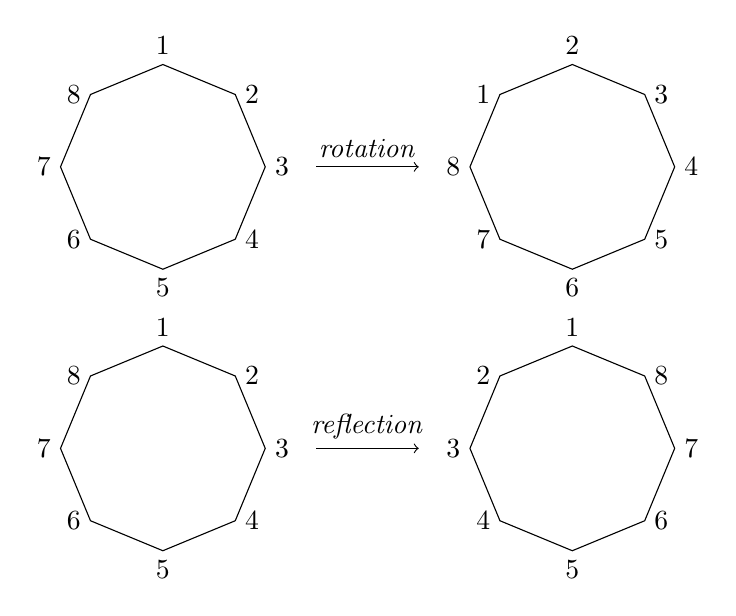
\begin{tikzpicture}[scale=1.3]

\draw (2,0)  +(45:1) node [right] {8} -- +(90:1) node [above] {1} -- +(135:1) node [left] {2} -- +(180:1) node [left] {3} -- +(225:1) node [left] {4} -- +(270:1) node [below] {5} -- +(315:1) node [right] {6} -- +(360:1) node [right] {7} -- cycle;

\draw (-2,0)  +(45:1) node [right] {2} -- +(90:1) node [above] {1} -- +(135:1) node [left] {8} -- +(180:1) node [left] {7} -- +(225:1) node [left] {6} -- +(270:1) node [below] {5} -- +(315:1) node [right] {4} -- +(360:1) node [right] {3} -- cycle;
\draw [->] (-0.5,0) -- (0.5,0);
\node [above] at (0,0) {\emph{reflection}};

\draw (2,2.75)  +(45:1) node [right] {3} -- +(90:1) node [above] {2} -- +(135:1) node [left] {1} -- +(180:1) node [left] {8} -- +(225:1) node [left] {7} -- +(270:1) node [below] {6} -- +(315:1) node [right] {5} -- +(360:1) node [right] {4} -- cycle;

\draw (-2,2.75)  +(45:1) node [right] {2} -- +(90:1) node [above] {1} -- +(135:1) node [left] {8} -- +(180:1) node [left] {7} -- +(225:1) node [left] {6} -- +(270:1) node [below] {5} -- +(315:1) node [right] {4} -- +(360:1) node [right] {3} -- cycle;

\draw [->] (-0.5,2.75) -- (0.5,2.75);
\node [above] at (0,2.75) {\emph{rotation}};

\end{tikzpicture}
\end{center}
\caption{Rotations and reflections of a regular $n$-gon}
\label{rotations}
\end{figure}

 
\begin{figure}[hbt]  %% Replaced with tikz figure and change to a counterclockwise rotation - TWJ 5/8/2010
\begin{center}
\tikzpreface{permute_reflections_ngon}
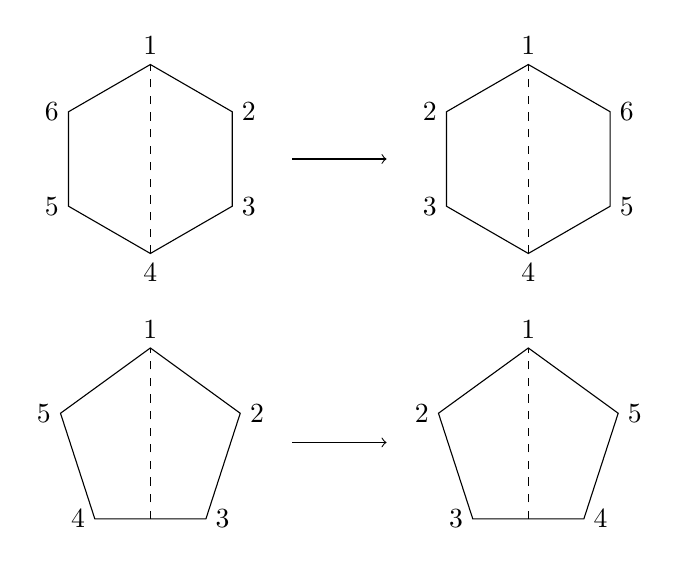
\begin{tikzpicture}[scale=1.2]

\draw (2,0)  +(18:1) node [right] {5} -- +(90:1) node [above] {1} -- +(162:1) node [left] {2} -- +(234:1) node [left] {3} -- +(306:1) node [right] {4} -- cycle;
\draw[dashed] (2,-0.80901) -- (2,1);

\draw (-2,0)  +(18:1) node [right] {2} -- +(90:1) node [above] {1} -- +(162:1) node [left] {5} -- +(234:1) node [left] {4} -- +(306:1) node [right] {3} -- cycle;
\draw[dashed] (-2,-0.80901) -- (-2,1);

\draw [->] (-0.5,0) -- (0.5,0);


\draw (2,3)  +(30:1) node [right] {6} -- +(90:1) node [above] {1} -- +(150:1) node [left] {2} -- +(210:1) node [left] {3} -- +(270:1) node [below] {4}  -- +(330:1) node [right] {5} -- cycle;
\draw[dashed] (2,2) -- (2,4);


\draw (-2,3)  +(30:1) node [right] {2} -- +(90:1) node [above] {1} -- +(150:1) node [left] {6} -- +(210:1) node [left] {5} -- +(270:1) node [below] {4}  -- +(330:1) node [right] {3} -- cycle;
\draw[dashed] (-2,2) -- (-2,4);

\draw [->] (-0.5,3) -- (0.5,3);


\end{tikzpicture}

\end{center}
\caption{Types of  reflections of a regular $n$-gon}
\label{types}
\end{figure}
 
 
 
\begin{theorem}\label{permute:Dn_generator_theorem}
The group $D_n$, $n \geq 3$, consists of all products of the two 
elements $r$ and $s$, satisfying the relations
\begin{align*}
r^n & = id \\
s^2 & = id \\
srs & = r^{-1}.
\end{align*}
\end{theorem}
 
 
%% TWJ, 2010/03/31
%% I think that this is a correct proof and simplified, but the proof needs to be checked.
\begin{proof}
The possible motions of a regular $n$-gon are either reflections or 
rotations (Figure~\ref{rotations}). There are exactly $n$ possible
rotations:
\[
id, \frac{360^{\circ} }{n}, 2 \cdot \frac{360^{\circ} }{n},
\ldots, (n-1) \cdot \frac{360^{\circ} }{n}.
\]
We will denote the rotation $360^{\circ} /n$ by $r$. The rotation $r$
generates all  of the other rotations. That is,
\[
r^k = k \cdot \frac{360^{\circ} }{n}.
\]
Label the $n$ reflections $s_1, s_2, \ldots, s_n$, where $s_k$ is the 
reflection that leaves vertex $k$ fixed. There are two cases of 
reflection, depending on whether $n$ is even or odd. If there are an 
even number of vertices, then 2 vertices are left fixed by a 
reflection. If there are an odd number of vertices, then only a single 
vertex is left fixed by a reflection (Figure~\ref{types}). 
%Hence, if $n = 2m$ for some integer $m$, then $s_i = s_{i+m}$ for $1 \leq i \leq m$. 
In either case, the order of $s_k$ is two. Let $s = s_1$. Then $s^2 = id$ and 
$r^n = id$. Since any rigid motion $t$ of the $n$-gon replaces the 
first vertex by the vertex $k$, the second vertex must be replaced 
by either $k+1$ or by $k-1$. If the second vertex is replaced by $k+1$, then $t = r^{k - 1}$.
If it is replaced by $k-1$, then $t = r^{k - 1} s$. Hence, $r$ and $s$
generate $D_n$; that is, $D_n$ consists of all finite products of $r$
and $s$. We will leave the proof that $srs = r^{-1}$ as an exercise.
\end{proof}
 
 
\begin{figure}[hbt]
\begin{center}

\tikzpreface{permute_dihedral_four}
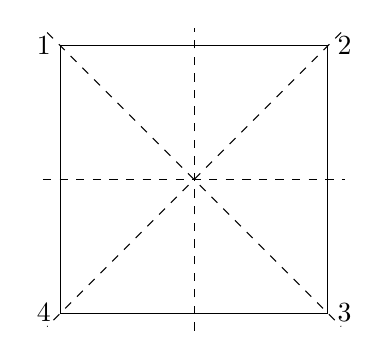
\begin{tikzpicture}[scale=1.2] %% Replaced with tikz figure and change to a counterclockwise rotation - TWJ 5/8/2010

\draw (0,0)  +(45:2) node [right] {2} -- +(135:2) node [left] {1} -- +(225:2) node [left] {4} -- +(315:2) node [right] {3} -- cycle;

\draw[dashed] (0,-1.6) -- (0,1.6);
\draw[dashed] (-1.6,0) -- (1.6,0);
\draw[dashed] (45:2.2) -- (225:2.2);
\draw[dashed] (135:2.2) -- (315:2.2);

\end{tikzpicture}
\end{center}
\caption{The group $D_4$}
\label{D4}
\end{figure}
 
 
\begin{example}{D4_group}
The group of rigid motions of a square, $D_4$, consists of eight
elements. With the vertices numbered 1, 2, 3, 4 (Figure~\ref{D4}), the 
rotations are 
\begin{align*}
r & = (1234) \\
r^2 & = (13)(24) \\
r^3 & = (1432) \\
r^4 & = id
\end{align*}
and the reflections are
\begin{align*}
s_1 & = (24) \\
s_2 & = (13).
\end{align*}
The order of $D_4$ is 8. The remaining two elements are
\begin{align*}
r s_1 & = (12)(34) \\
r^3 s_1 & = (14)(23).
\end{align*}
\end{example}
 
 
 
\begin{figure}[hbt]
\begin{center}
\tikzpreface{permute_motions_cube}
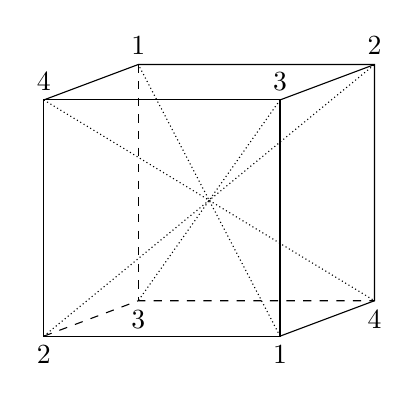
\begin{tikzpicture}[scale=1.5] %% Replaced with tikz figure and change to a counterclockwise rotation - TWJ 5/8/2010

\draw (0,0)  -- (0,2) -- (2,2) -- (2,0) -- cycle;
\draw (0,2)  -- (0.8,2.3) -- (2.8,2.3) -- (2.8,0.3) -- (2,0);
\draw (2,2) -- (2.8,2.3);
\draw[dashed] (0,0) -- (0.8,0.3) -- (2.8,0.3);
\draw[dashed] (0.8,2.3) -- (0.8,0.3);

\draw[densely dotted] (0,0) node [below] {2}-- (2.8,2.3) node [above] {2};
\draw[densely dotted] (0,2) node [above] {4} -- (2.8,0.3) node [below] {4};
\draw[densely dotted] (2,0) node [below] {1} -- (0.8,2.3) node [above] {1};
\draw[densely dotted] (2,2) node [above] {3} -- (0.8,0.3) node [below] {3};


\end{tikzpicture}

\end{center}
\caption{The motion group of a cube}
\label{motions}
\end{figure}
 
 
 
 
\subsection*{The Motion Group of a Cube}
 
 
We can investigate the groups of rigid motions of  geometric
objects other than a regular $n$-sided polygon to obtain interesting
examples of permutation groups. Let us consider the group of rigid
motions of a cube. One of the first questions that we can ask about
this group is ``what is its order?''  A cube has 6 sides. If
a particular side is facing upward, then there are four possible
rotations of the cube that will preserve the upward-facing side.
Hence, the order of the group is $6 \cdot 4 = 24$. We have just proved
the following proposition.
 
 
\begin{proposition}\label{motions_cube}
The group of rigid motions of a cube contains $24$ elements.
\end{proposition}
 
 
\begin{theorem}
The group of rigid motions of a cube is $S_4$.
\end{theorem}
 

 
\begin{figure}[hbt]
\begin{center}
\tikzpreface{permute_transpositions_cube}
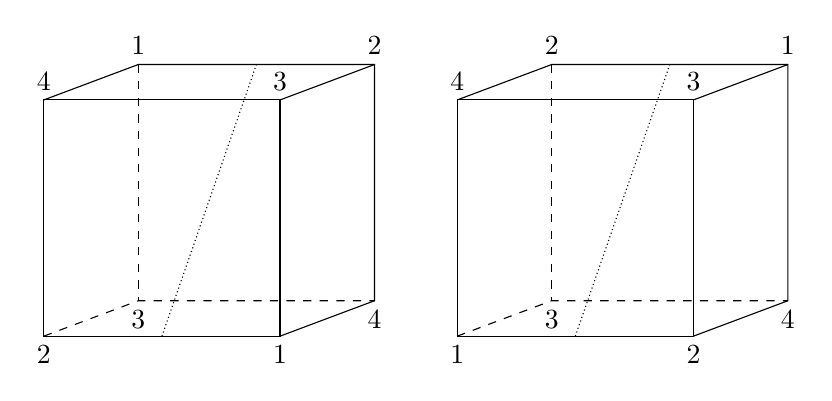
\begin{tikzpicture}[scale=1.5] %% Replaced with tikz figure and change to a counterclockwise rotation - TWJ 5/8/2010

\draw (0,0) node [below] {2} -- (0,2) node [above] {4} -- (2,2) node [above] {3}-- (2,0) node [below] {1} -- cycle;
\draw (0,2)  -- (0.8,2.3) node [above] {1} -- (2.8,2.3) node [above] {2}-- (2.8,0.3) node [below] {4} -- (2,0);
\draw (2,2) -- (2.8,2.3);
\draw[dashed] (0,0) -- (0.8,0.3) -- (2.8,0.3);
\draw[dashed] (0.8,2.3) -- (0.8,0.3)  node [below] {3};

\draw[densely dotted] (1,0) -- (1.8,2.3);

\draw (3.5,0) node [below] {1} -- (3.5,2) node [above] {4} -- (5.5,2) node [above] {3}-- (5.5,0) node [below] {2} -- cycle;
\draw (3.5,2)  -- (4.3,2.3) node [above] {2} -- (6.3,2.3) node [above] {1}-- (6.3,0.3) node [below] {4} -- (5.5,0);
\draw (5.5,2) -- (6.3,2.3);
\draw[dashed] (3.5,0) -- (4.3,0.3) -- (6.3,0.3);
\draw[dashed] (4.3,2.3) -- (4.3,0.3) node [below] {3};

\draw[densely dotted] (4.5,0) -- (5.3,2.3);

\end{tikzpicture}

\end{center}
\caption{Transpositions in the motion group of a cube}
\label{transpose}
\end{figure}
 
 

 
\begin{proof}
From Proposition~\ref{motions_cube}, we already know that the motion group of the
cube has 24 elements, the same number of elements as there are in
$S_4$.  There are exactly four diagonals in the cube.  If we label
these diagonals 1, 2, 3, and 4, we must show that the motion group of
the cube will give us any permutation of the diagonals
(Figure~\ref{motions}). If we can obtain all of these permutations,
then $S_4$ and the group of rigid motions of the cube must be the
same. To obtain a transposition we can rotate the cube $180^{\circ}$
about the axis joining the midpoints of opposite edges
(Figure~\ref{transpose}). There are six such axes, giving all
transpositions in $S_4$. Since every element in $S_4$ is the product
of a finite number of transpositions, the motion group of a cube
must be $S_4$.
\hspace*{1in}
\end{proof}
 

 
 
\markright{EXERCISES}
\section*{Exercises}
\exrule
 
 
 
{\small
\begin{enumerate}
 
%*****************Calculations********************
 
 
\item %1
Write the following permutations in cycle notation.
\begin{multicols}{2}
\begin{enumerate}
 
\item
\[
\begin{pmatrix}
1 & 2 & 3 & 4 & 5 \\
2 & 4 & 1 & 5 & 3
\end{pmatrix}
\]

\item
\[
\begin{pmatrix}
1 & 2 & 3 & 4 & 5 \\
4 & 2 & 5 & 1 & 3
\end{pmatrix}
\]

\item
\[
\begin{pmatrix}
1 & 2 & 3 & 4 & 5 \\
3 & 5 & 1 & 4 & 2
\end{pmatrix}
\]

\item
\[
\begin{pmatrix}
1 & 2 & 3 & 4 & 5 \\
1 & 4 & 3 & 2 & 5
\end{pmatrix}
\]

\end{enumerate}
\end{multicols}


 
 \item  %2
Compute each of the following.
\begin{multicols}{2}
\begin{enumerate}
 
\item
$(1345)(234)$
  
\item
$(12)(1253)$

\item
$(143)(23)(24)$

\item
$(1423)(34)(56)(1324)$

\item
$(1254)(13)(25)$

 
\item
$(1254) (13)(25)^2$
 
\item
$(1254)^{-1} (123)(45) (1254)$
  
\item
$(1254)^2 (123)(45)$
 
\item
$(123)(45) (1254)^{-2}$

\item
$(1254)^{100}$
 
\item
$|(1254)|$

  
\item
$|(1254)^2|$
  
\item
$(12)^{-1}$

\item
$(12537)^{-1}$
 
\item
$[(12)(34)(12)(47)]^{-1}$

\item
$[(1235)(467)]^{-1}$
 
\end{enumerate}
\end{multicols}
 
 
 \item %3
Express the following permutations as products of transpositions and
identify them as even or odd. 
\begin{multicols}{2}
\begin{enumerate}
 
\item
$(14356)$

 \item
$(156)(234)$
 
 \item
$(1426)(142)$
 
 \item
$(17254)(1423)(154632)$
 
 \item
$(142637)$
 
\end{enumerate}
\end{multicols}


 
\item %5
Find $(a_1, a_2, \ldots, a_n)^{-1}$.
 
\item %6
List all of the subgroups of $S_4$. Find each of the following sets. 
\begin{enumerate}
 
 \item
$\{ \sigma \in S_4 : \sigma(1) = 3 \}$
 
 \item
$\{ \sigma \in S_4 : \sigma(2) = 2 \}$
 
 \item
$\{ \sigma \in S_4 : \sigma(1) = 3 \mbox{ and } \sigma(2) =
2 \}$
 
\end{enumerate}
Are any of these sets subgroups of $S_4$?
 
 
\item
Find all of the subgroups in $A_4$. What is the order of each
subgroup? 
 
 
\item
Find all possible orders of elements in $S_7$ and $A_7$.
 
 
\item
Show that $A_{10}$ contains an element of order 15.
 
 
\item
Does $A_8$ contain an element of order 26?
 
 
\item %7
Find an element of largest order in $S_n$ for $n = 3, \ldots, 10$. 
 
 
\item
What are the possible cycle structures of elements of $A_5$? What
about $A_6$? 
 
 
\item
Let $\sigma \in S_n$ have order $n$. Show that for all integers $i$
and $j$, $\sigma^i = \sigma^j$ if and only if $i \equiv j \pmod{n}$. 
 
 
\item\label{permute:OrderProductCycles}
Let $\sigma = \sigma_1 \cdots \sigma_m \in S_n$ be the product of
disjoint cycles. Prove that the order of $\sigma$ is the least common
multiple of the lengths of the cycles $\sigma_1, \ldots, \sigma_m$.
 
 
\item
Using cycle notation, list the elements in $D_5$.  What are $r$ and
$s$?  Write every element as a product of $r$ and $s$.
 
 
\item
If the diagonals of a cube are labeled as Figure~\ref{motions}, to
which motion of the cube does the permutation $(12)(34)$ correspond?
What about the other permutations of the diagonals?
 
 
\item
Find the group of rigid motions of a tetrahedron.  Show that this is
the same group as $A_4$. 
 
 
%******************************Theory********************
 
 
\item
Prove that $S_n$ is nonabelian for $n \geq 3$.
 
 
\item
Show that $A_n$ is nonabelian for $n \geq 4$.
 
 
\item
Prove that $D_n$ is nonabelian for $n \geq 3$.
 
 
\item
Let $\sigma \in S_n$. Prove that $\sigma$ can be written as the
product of at most $n-1$ transpositions. 
 
 
\item
Let $\sigma \in S_n$. If $\sigma$ is not a cycle, prove that $\sigma$
can be written as the product of at most $n-2$ transpositions.
 
 
\item
If $\sigma$ can be expressed as an odd number of transpositions, show
that any other product of transpositions equaling $\sigma$ must also
be odd. 
 
 
\item
If $\sigma$ is a cycle of odd length, prove that $\sigma^2$ is also a
cycle. 
 
 
\item
Show that a 3-cycle is an even permutation.
 
 
\item
Prove that in $A_n$ with $n \geq 3$, any permutation is a product of
cycles of length~3.  
 
 
\item
Prove that any element in $S_n$ can be written as a finite product of
the following permutations.
\begin{enumerate}
 
 \item
$(1 2), (13), \ldots, (1n)$
 
 \item
$(1 2), (23), \ldots, (n- 1,n)$
 
 \item
$(12), (1 2 \ldots n )$
 
\end{enumerate}
 
 
\item
Let $G$ be a group and define a map $\lambda_g : G \rightarrow G$ by
$\lambda_g(a) = g a$.  Prove that $\lambda_g$ is a permutation of $G$.
 
 
 
\item
Prove that there exist $n!$ permutations of a set containing $n$
elements. 
 
 
\item
Recall that the \boldemph{center}\index{Group!center of} of a group $G$ is
\[
Z(G) = \{ g \in G : \mbox{$gx = xg$ for all $x \in G$} \}.
\]
Find the center of $D_8$. What about the center of $D_{10}$? What is
the center of $D_n$? 
 
 
\item
Let $\tau = (a_1, a_2, \ldots, a_k)$ be a cycle of length $k$.
\begin{enumerate}
 
 \item
Prove that if $\sigma$ is any permutation, then
\[
\sigma \tau \sigma^{-1 } = ( \sigma(a_1), \sigma(a_2), \ldots,
\sigma(a_k))
\]
is a cycle of length $k$.
 
 \item
Let $\mu$ be a cycle of length $k$. Prove that there is a permutation
$\sigma$ such that $\sigma \tau \sigma^{-1 } = \mu$.
 
\end{enumerate}
 
 
\item
For $\alpha$ and $\beta$ in $S_n$, define $\alpha \sim \beta$ if there
exists an $\sigma \in S_n$ such that $\sigma \alpha \sigma^{-1} =
\beta$.  Show that $\sim$ is an equivalence relation on $S_n$.
 
 
\item
Let $\sigma \in S_X$. If $\sigma^n(x) = y$, we will say that $x \sim
y$. 
\begin{enumerate}
 
 \item
Show that $\sim$ is an equivalence relation on $X$.
 
 \item
If $\sigma \in A_n$ and $\tau \in S_n$, show that $\tau^{-1} \sigma
\tau \in A_n$. 
 
\item
Define the \boldemph{orbit}\index{Orbit} of $x \in X$ under $\sigma \in
S_X$ to be the set 
\[
{\mathcal O}_{x, \sigma} = \{ y : x \sim y  \}.
\]
Compute the orbits of $\alpha, \beta, \gamma$ where
\begin{align*}
\alpha & = (1254) \\
\beta & = (123)(45)\\
\gamma & = (13)(25).
\end{align*}
 
 \item
If ${\mathcal O}_{x, \sigma} \cap {\mathcal O}_{y, \sigma} \neq \emptyset$,
prove that ${\mathcal O}_{x, \sigma} = {\mathcal O}_{y, \sigma}$.  The orbits
under a permutation $\sigma$ are the equivalence classes corresponding
to the equivalence relation $\sim$.
 
 
\item
A subgroup $H$ of $S_X$ is \boldemph{
transitive}\index{Subgroup!transitive} if for every $x, y \in X$, 
there exists a $\sigma \in H$ such that $\sigma(x) =y$. Prove that
$\langle \sigma \rangle$ is transitive if and only if ${\mathcal O}_{x,
\sigma} = X$ for some $x \in X$. 
 
 
\end{enumerate}
 
 
\item
Let $\alpha \in S_n$ for $n \geq 3$. If $\alpha \beta = \beta \alpha$
for all $\beta \in S_n$, prove that $\alpha$ must be the identity
permutation; hence, the center of $S_n$ is the trivial subgroup. 
 
 
\item
If $\alpha$ is even, prove that $\alpha^{-1}$ is also even. Does a
corresponding result hold if $\alpha$ is odd? 
 
 
\item
Show that  $\alpha^{-1} \beta^{-1} \alpha \beta$ is even for $\alpha,
\beta \in S_n$. 
 
 
\item
Let $r$ and $s$ be the elements in $D_n$ described in Theorem~\ref{permute:Dn_generator_theorem}.
\begin{enumerate}
 
 \item
Show that $srs = r^{-1}$.
 
 \item
Show that $r^k s = s r^{-k}$ in $D_n$.
 
 \item
Prove that the order of $r^k \in D_n$ is $n / \gcd(k,n)$.
  
\end{enumerate}
 
 
\end{enumerate}
}
 
\sagesection
 
